%==============================================================================
% Figure: 3D Aether Crystalline Lattice
% Purpose: Visualize crystalline spacetime structure with defects
% Chapter: Ch09 - Aether Crystalline Structure
% Type: Schematic
%==============================================================================

\begin{figure}[htbp]
  \centering
  \begin{tikzpicture}[
    scale=1.0,
    x={(0.866cm, -0.5cm)},
    y={(0.866cm, 0.5cm)},
    z={(0cm, 1cm)},
    lattice/.style={circle, draw=black, fill=blue!30, thick, minimum size=4mm},
    defect/.style={circle, draw=red, fill=red!50, thick, minimum size=5mm},
    perturbation/.style={circle, draw=orange, fill=orange!30, thick, minimum size=4mm},
    bond/.style={thick, gray!60}
  ]

    % Define lattice dimensions
    \def\nx{4}
    \def\ny{4}
    \def\nz{3}

    % Draw bonds first (behind nodes)
    \foreach \x in {0,...,\nx} {
      \foreach \y in {0,...,\ny} {
        \foreach \z in {0,...,\nz} {
          % x-direction bonds
          \ifnum\x<\nx
            \draw[bond] (\x, \y, \z) -- ({\x+1}, \y, \z);
          \fi
          % y-direction bonds
          \ifnum\y<\ny
            \draw[bond] (\x, \y, \z) -- (\x, {\y+1}, \z);
          \fi
          % z-direction bonds
          \ifnum\z<\nz
            \draw[bond] (\x, \y, \z) -- (\x, \y, {\z+1});
          \fi
        }
      }
    }

    % Draw lattice nodes
    \foreach \x in {0,...,\nx} {
      \foreach \y in {0,...,\ny} {
        \foreach \z in {0,...,\nz} {
          % Regular lattice nodes
          \node[lattice] at (\x, \y, \z) {};
        }
      }
    }

    % Add defect (vacancy)
    \node[defect] (defect1) at (2, 2, 1) {};
    \node[font=\tiny, below=0.1cm of defect1, text=red] {Vacancy};

    % Add perturbation (displaced node)
    \node[perturbation] at (3.2, 1.8, 2) {};
    \draw[->, >=stealth, ultra thick, orange] (3, 2, 2) -- (3.2, 1.8, 2);
    \node[font=\tiny, above right, text=orange] at (3.2, 1.8, 2) {Displacement};

    % Add interstitial defect
    \node[defect] (defect2) at (1.5, 3.5, 1.5) {};
    \node[font=\tiny, above=0.1cm of defect2, text=red] {Interstitial};

    % Highlight unit cell
    \draw[ultra thick, blue!70, dashed]
      (0, 0, 0) -- (1, 0, 0) -- (1, 1, 0) -- (0, 1, 0) -- cycle;
    \draw[ultra thick, blue!70, dashed]
      (0, 0, 1) -- (1, 0, 1) -- (1, 1, 1) -- (0, 1, 1) -- cycle;
    \draw[ultra thick, blue!70, dashed]
      (0, 0, 0) -- (0, 0, 1);
    \draw[ultra thick, blue!70, dashed]
      (1, 0, 0) -- (1, 0, 1);
    \draw[ultra thick, blue!70, dashed]
      (1, 1, 0) -- (1, 1, 1);
    \draw[ultra thick, blue!70, dashed]
      (0, 1, 0) -- (0, 1, 1);

    \node[font=\small, text=blue!70, align=center] at (0.5, 0.5, -0.8) {Unit cell\\$a \sim \ell_{\text{Pl}}$};

    % Basis vectors
    \draw[->, >=stealth, ultra thick, black] (0, 0, 0) -- (1.5, 0, 0) node[right] {$\mathbf{a}_1$};
    \draw[->, >=stealth, ultra thick, black] (0, 0, 0) -- (0, 1.5, 0) node[right] {$\mathbf{a}_2$};
    \draw[->, >=stealth, ultra thick, black] (0, 0, 0) -- (0, 0, 1.5) node[above] {$\mathbf{a}_3$};

    % Phonon wave annotation
    \draw[->, >=stealth, ultra thick, green!60!black, decorate, decoration={snake, amplitude=2mm, segment length=5mm}]
      (0, \ny, \nz) -- (\nx, \ny, \nz)
      node[midway, above, font=\small, align=center] {Phonon\\(graviton)};

    % Title
    \node[anchor=south, font=\Large\bfseries] at (2, 0, 5) {Aether Crystalline Lattice (3D)};

  \end{tikzpicture}

  % Annotations below diagram
  \vspace{0.5cm}

  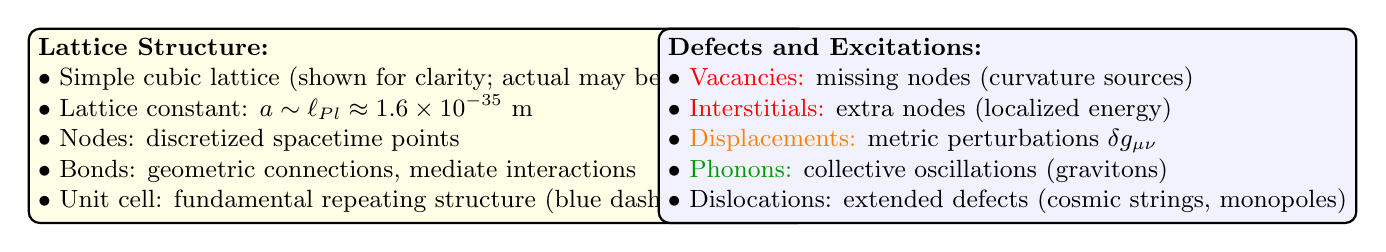
\begin{tikzpicture}
    \node[anchor=north west, align=left, font=\small, draw=black, fill=yellow!10, rounded corners, thick]
      at (0, 0) {
      \textbf{Lattice Structure:} \\
      $\bullet$ Simple cubic lattice (shown for clarity; actual may be FCC/BCC) \\
      $\bullet$ Lattice constant: $a \sim \ell_{\text{Pl}} \approx 1.6 \times 10^{-35}$ m \\
      $\bullet$ Nodes: discretized spacetime points \\
      $\bullet$ Bonds: geometric connections, mediate interactions \\
      $\bullet$ Unit cell: fundamental repeating structure (blue dashed)
    };

    \node[anchor=north west, align=left, font=\small, draw=black, fill=blue!5, rounded corners, thick]
      at (8, 0) {
      \textbf{Defects and Excitations:} \\
      $\bullet$ \textcolor{red}{Vacancies:} missing nodes (curvature sources) \\
      $\bullet$ \textcolor{red}{Interstitials:} extra nodes (localized energy) \\
      $\bullet$ \textcolor{orange}{Displacements:} metric perturbations $\delta g_{\mu\nu}$ \\
      $\bullet$ \textcolor{green!60!black}{Phonons:} collective oscillations (gravitons) \\
      $\bullet$ Dislocations: extended defects (cosmic strings, monopoles)
    };
  \end{tikzpicture}

  \caption{Three-dimensional representation of the Aether crystalline spacetime lattice. The
    fundamental structure consists of a regular lattice with spacing $a \sim \ell_{\text{Pl}}$
    (Planck length), where nodes represent discretized spacetime points and bonds encode geometric
    relationships. The blue dashed cube highlights a single unit cell with basis vectors
    $\mathbf{a}_1, \mathbf{a}_2, \mathbf{a}_3$. Defects play a crucial role: vacancies (red,
    missing nodes) source spacetime curvature (Einstein equations as elasticity); interstitials
    (red, extra nodes) represent localized energy concentrations; displacements (orange) are
    metric perturbations $\delta g_{\mu\nu}$. Collective oscillations (green wavy arrow) are
    phonon modes, which in the long-wavelength limit reproduce gravitons. This crystalline
    picture provides a microscopic foundation for general relativity, with the Einstein-Hilbert
    action emerging as an effective low-energy description of lattice elasticity.}
  \label{fig:crystalline-lattice-3d}
\end{figure}
